\documentclass[border=2pt]{standalone}
\usepackage{tikz}
\usetikzlibrary{arrows,shapes.geometric}
\begin{document}
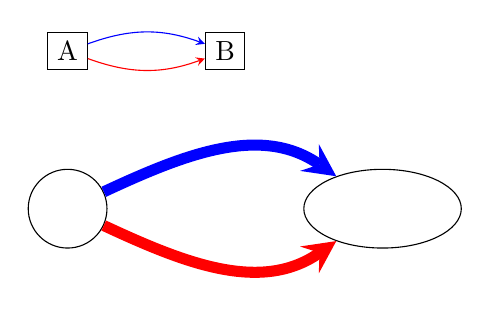
\begin{tikzpicture}
  \node[draw,minimum width=.5cm,minimum height=.3cm] (a) at (0,0) {A};
  \node[draw,minimum width=.5cm,minimum height=.3cm] (b) at (2,0) {B};
  \draw[-stealth,blue] (a) to[out=20,in=160] (b);
  \draw[-stealth,red] (a) to[out=-20,in=200] (b);
  \node[draw,circle,minimum size=1cm,inner sep=0pt] (c) at (0,-2) {};
  \node[draw,ellipse,minimum width=2cm,minimum height=1cm,inner sep=0pt] (d) at (4,-2) {};
  \draw[line width=4pt,-stealth,blue] (c) to[out=25,in=145] (d);
  \draw[line width=4pt,-stealth,red] (c.-25) to[out=-25,in=215] (d.215);
\end{tikzpicture}
\end{document}
